\documentclass[conference]{IEEEtran}

\usepackage{graphicx}
\usepackage{booktabs}
\usepackage{caption}
\usepackage{subcaption}
\usepackage{amsmath}
\usepackage{hyperref}
\usepackage{float}

\begin{document}

\title{EE 576 Project 4: Time-Varying Images and Optical Flow}

\author{\IEEEauthorblockN{Abdulhalim Kiraz}
\IEEEauthorblockA{Student ID: 2021401219\\
abdulhalim.kiraz@std.bogazici.edu.tr}}

\maketitle

\thispagestyle{empty}
\pagestyle{empty}

\begin{abstract}
In this project, dense optical flow and sparse feature tracking were applied to image sequences. Farneback optical flow was used for dense motion estimation. For sparse motion estimation, SIFT keypoints were tracked with Lucas-Kanade optical flow. The results were compared by looking at the output images, the average direction similarity, and the average flow differences in moving regions.
\end{abstract}

\section{Introduction and Methodology}

The program shows the results in a $2 \times 2$ display. The top row contains frame $n$ and frame $n+1$. The bottom-left cell shows the dense optical flow result. The bottom-right cell shows sparse SIFT + Lucas-Kanade tracking.

For dense optical flow, consecutive frames were converted to grayscale. Then OpenCV Farneback optical flow was computed. For the TUM sequence, the given mask images were used to find moving regions. Connected components were found from the mask, and the average dense flow vector was drawn on each region.

For sparse optical flow, SIFT keypoints were detected in the first frame. These points were tracked to the next frame with pyramidal Lucas-Kanade optical flow. The result was drawn as point tracks. For the mask regions, SIFT points were also detected inside each region. In this way, the average sparse vector could be compared with the average dense vector.

The second dataset was the kitchen sequence. This dataset did not have mask images. Therefore, a simple automatic mask was produced using frame difference. The absolute difference between two grayscale frames was blurred, thresholded, and cleaned with morphology.

The dense and sparse methods were compared in two ways. First, average orientation similarity was computed by comparing sparse track vectors with dense flow vectors at the same positions. Second, for moving regions, the norm between dense and sparse average vectors was reported.

\section{Results}

Two frame pairs were selected from the TUM sequence. In the figures, yellow regions show the moving masks. Red arrows show dense average flow, green arrows show sparse tracks, and blue arrows show average sparse region flow.

\begin{figure}[H]
    \centering
    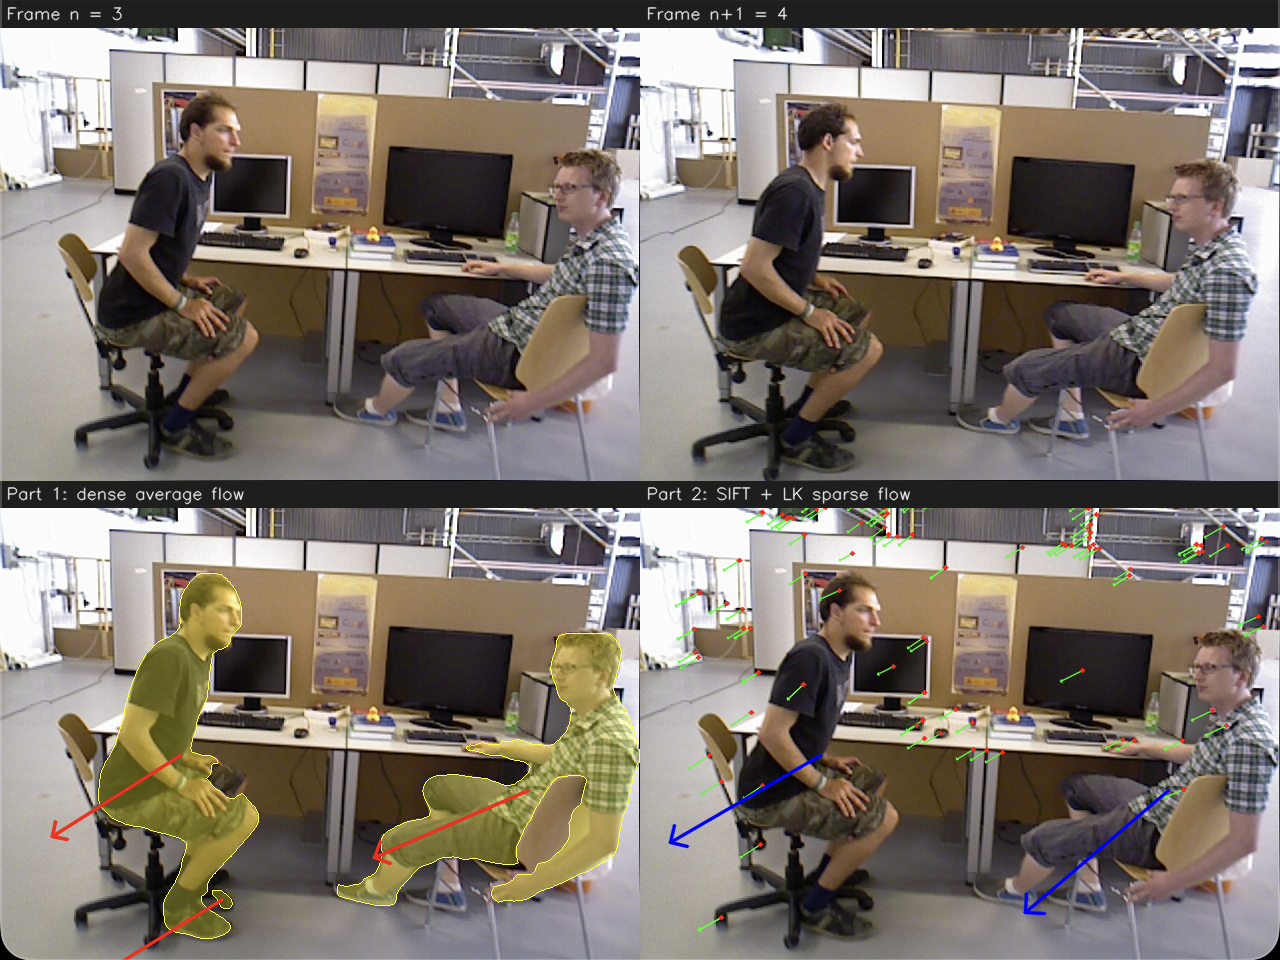
\includegraphics[width=0.85\linewidth]{report_assets/figures/frame_3_4_grid.png}
    \caption{TUM frames 3--4.}
    \label{fig:tum34}
\end{figure}




\begin{table}[H]
\centering
\caption{Orientation comparison between dense and sparse flow.}
\label{tab:orientation}
\renewcommand{\arraystretch}{1.12}
\begin{tabular}{l c c c c}
\toprule
\textbf{Dataset} & \textbf{Frames} & \textbf{Tracks} & \textbf{Cosine} & \textbf{Angle} \\
\midrule
TUM & 3--4 & 120 & 0.995 & 1.247$^\circ$ \\
TUM & 45--46 & 120 & 0.988 & 1.744$^\circ$ \\
Kitchen & 15--16 & 120 & 0.880 & 14.233$^\circ$ \\
Kitchen & 89--90 & 120 & 0.975 & 3.522$^\circ$ \\
\bottomrule
\end{tabular}
\end{table}





The TUM results have high cosine similarity. This means that the dense and sparse methods mostly give similar motion directions for these frame pairs.



\begin{figure}[H]
    \centering
    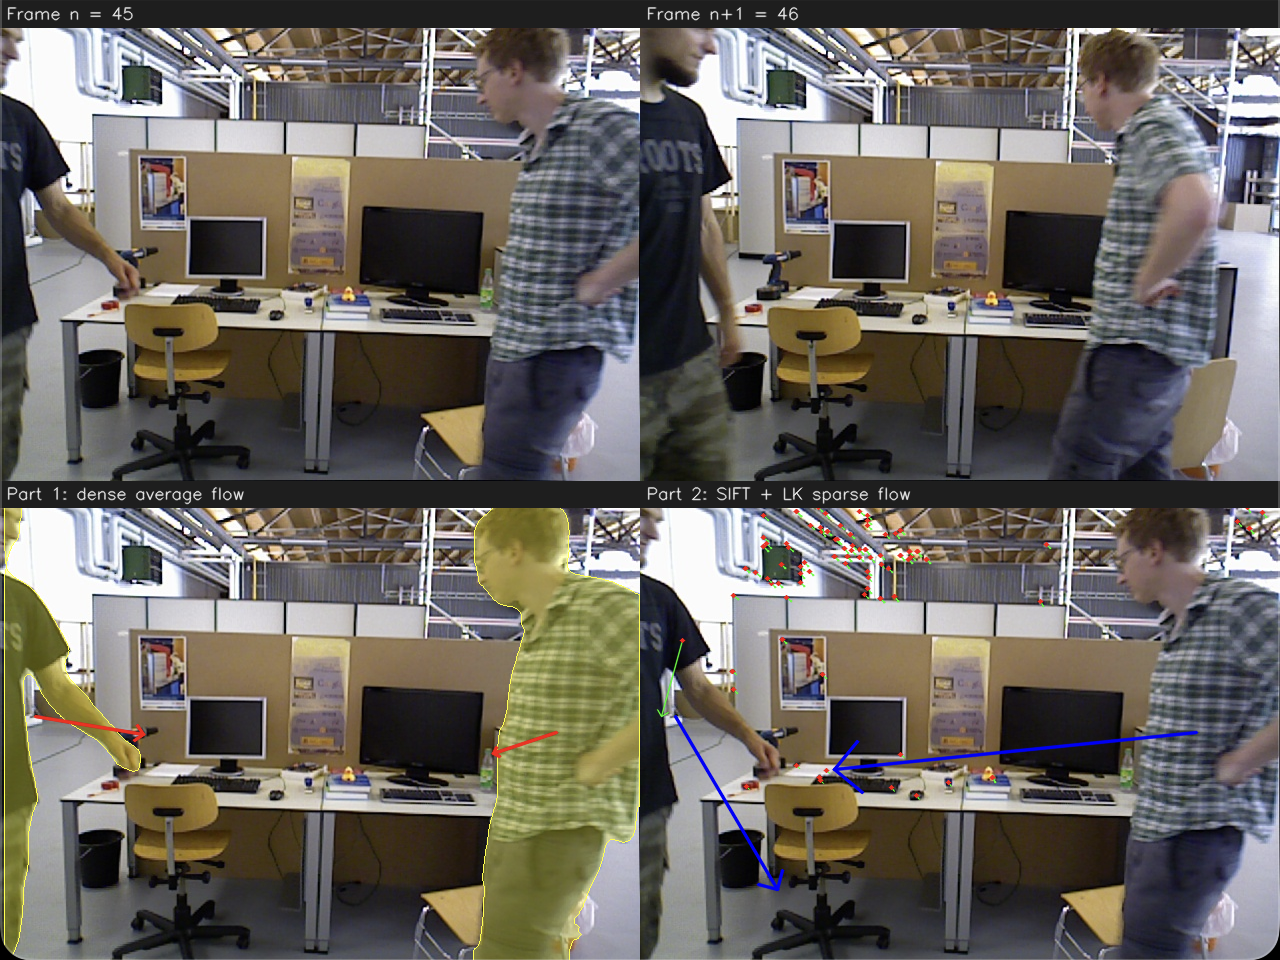
\includegraphics[width=0.85\linewidth]{report_assets/figures/frame_45_46_grid.png}
    \caption{TUM frames 45--46.}
    \label{fig:tum4546}
\end{figure}

\begin{table*}[t]
\centering
\caption{TUM region-based dense and sparse average flow comparison.}
\label{tab:tumregions}
\renewcommand{\arraystretch}{1.12}
\begin{tabular}{c c c c c c}
\toprule
\textbf{Frames} & \textbf{Region} & \textbf{Tracks} & \textbf{Dense Avg. Flow} & \textbf{Sparse Avg. Flow} & \textbf{Norm} \\
\midrule
3--4 & 1 & 8 & $(-15.935,\;10.037)$ & $(-18.718,\;10.865)$ & 2.904 \\
3--4 & 2 & 11 & $(-19.167,\;8.375)$ & $(-17.843,\;15.320)$ & 7.071 \\
45--46 & 1 & 5 & $(13.450,\;2.210)$ & $(12.716,\;21.544)$ & 19.348 \\
45--46 & 2 & 2 & $(-7.766,\;2.574)$ & $(-45.255,\;4.560)$ & 37.542 \\
\bottomrule
\end{tabular}
\end{table*}

For frames 3--4, the region differences are smaller. For frames 45--46, the differences are larger. The main reason is that only a few sparse tracks were found inside some regions.

The kitchen dataset was used as a second sequence. The same dense and sparse methods were applied. The only difference was that the moving masks were generated automatically by frame difference.

\begin{figure}[H]
    \centering
    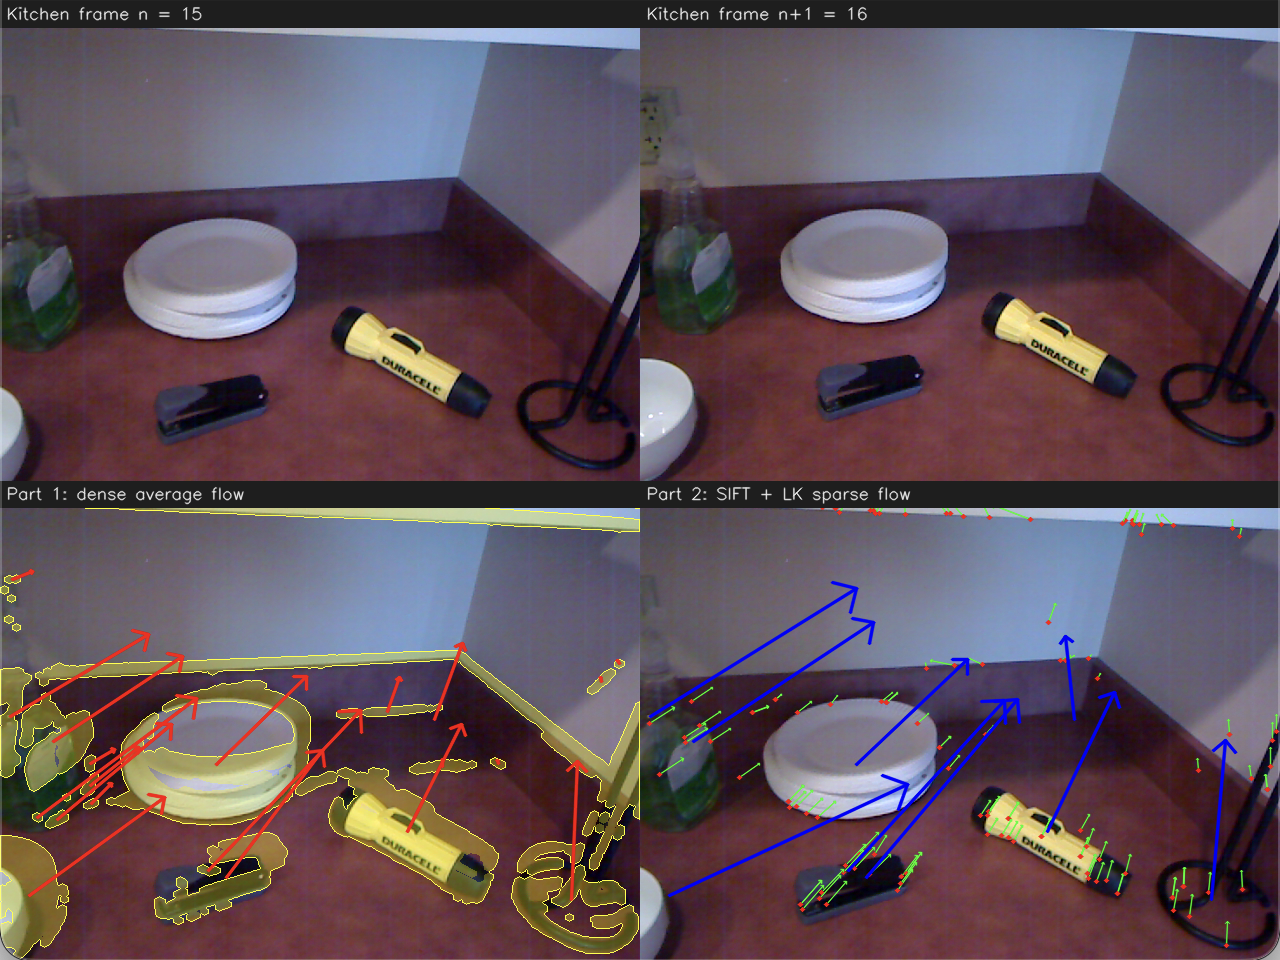
\includegraphics[width=0.95\linewidth]{report_assets/figures/kitchen_frame_n15.png}
    \caption{Kitchen frames 15--16.}
    \label{fig:kitchen15}
\end{figure}

\begin{figure}[H]
    \centering
    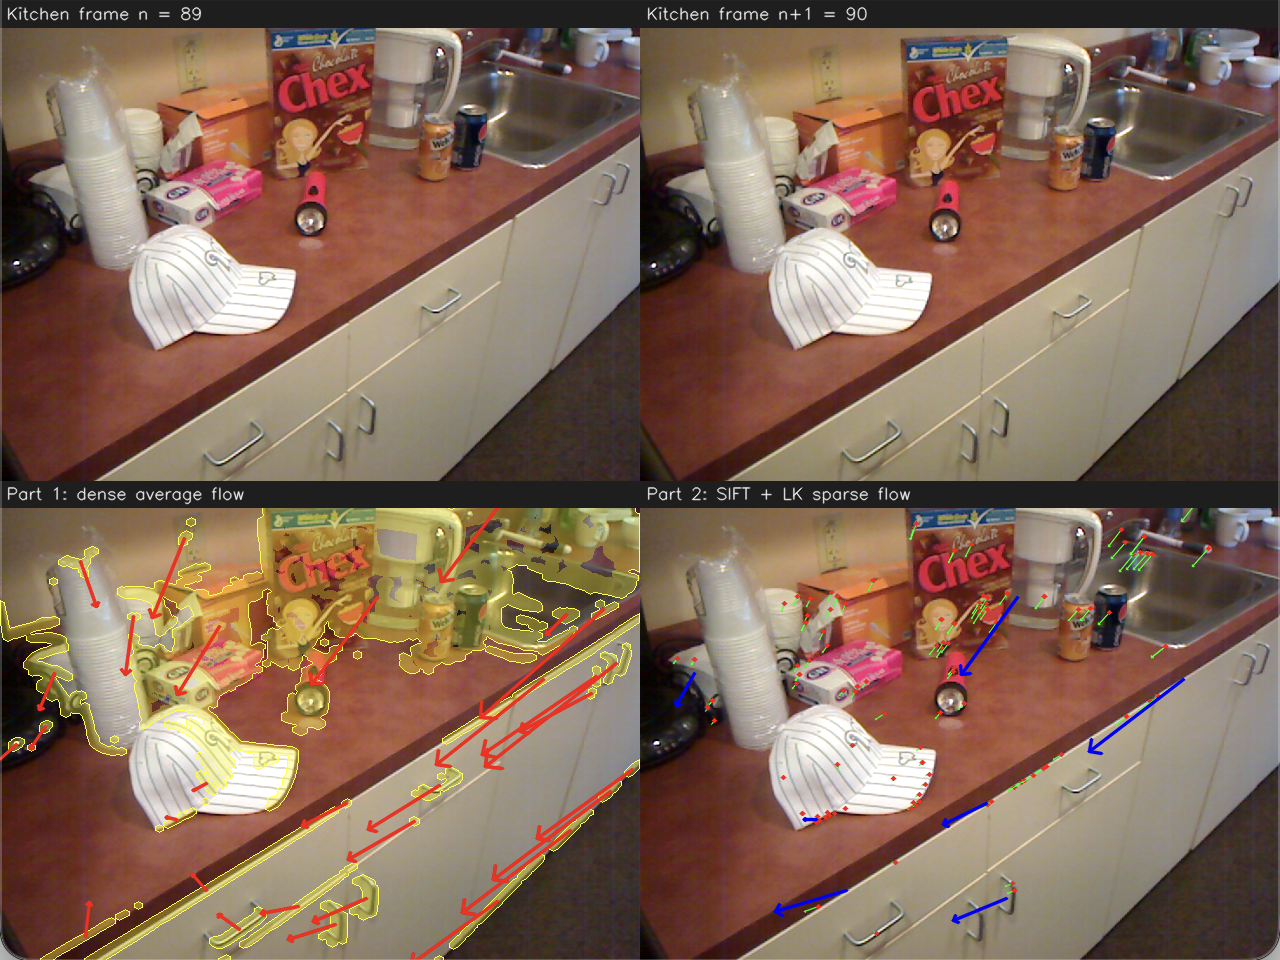
\includegraphics[width=0.95\linewidth]{report_assets/figures/kitchen_frame_n89.png}
    \caption{Kitchen frames 89--90.}
    \label{fig:kitchen89}
\end{figure}

\begin{table}[H]
\centering
\caption{Kitchen automatic mask summary.}
\label{tab:kitchen}
\renewcommand{\arraystretch}{1.12}
\begin{tabular}{c c c c c}
\toprule
\textbf{Frames} & \textbf{Regions} & \textbf{Compared} & \textbf{Min Norm} & \textbf{Max Norm} \\
\midrule
15--16 & 22 & 11 & 1.418 & 31.444 \\
89--90 & 30 & 7 & 0.087 & 8.490 \\
\bottomrule
\end{tabular}
\end{table}

\section{Evaluation and Discussion}

Dense optical flow gave a stable summary for moving regions, especially when the mask was already available. Sparse tracking was easier to inspect visually. However, it depended on the number and quality of SIFT tracks. When only a few tracks were found inside a region, the average sparse vector became less reliable.

The kitchen results show the limitation of the automatic mask. Frame difference finds many changed regions, but some of them are small or noisy. Because of this, frames 15--16 had a larger average angle difference. Frames 89--90 gave a better result, with cosine similarity 0.975 and average angle difference 3.522 degrees.

\section{Conclusion}

Dense and sparse optical flow methods were implemented and compared on two image sequences. The TUM sequence gave cleaner region results because mask images were available. The kitchen sequence was processed by generating simple frame-difference masks. In general, dense and sparse flow directions were similar in the selected examples. Region differences became larger when the sparse method had too few reliable tracks.

\section*{AI Usage Declaration}

ChatGPT/Codex (May 2026) was used as a supportive tool
for code debugging.

\begin{thebibliography}{9}

\bibitem{optflow}
H.~I.~Bozma, ``EE 576 -- Optical Flow,'' Lecture slides, Bogazici University.

\bibitem{tracking}
H.~I.~Bozma, ``EE 576 -- Tracking,'' Lecture slides, Bogazici University.

\bibitem{farneback}
G.~Farneback, ``Two-frame motion estimation based on polynomial expansion,'' in \textit{Proc. Scandinavian Conference on Image Analysis}, 2003.

\bibitem{lk}
B.~D.~Lucas and T.~Kanade, ``An iterative image registration technique with an application to stereo vision,'' in \textit{Proc. IJCAI}, 1981.

\bibitem{sift}
D.~G.~Lowe, ``Distinctive image features from scale-invariant keypoints,'' \textit{International Journal of Computer Vision}, 2004.

\bibitem{opencv}
OpenCV Contributors, ``OpenCV: Open Source Computer Vision Library.'' [Online]. Available: \url{https://opencv.org/}

\end{thebibliography}

\end{document}
